\documentclass[11pt,]{article}
\usepackage[left=1in,top=1in,right=1in,bottom=1in]{geometry}
\newcommand*{\authorfont}{\fontfamily{phv}\selectfont}
\usepackage[]{mathpazo}


  \usepackage[T1]{fontenc}
  \usepackage[utf8]{inputenc}



\usepackage{abstract}
\renewcommand{\abstractname}{}    % clear the title
\renewcommand{\absnamepos}{empty} % originally center

\renewenvironment{abstract}
 {{%
    \setlength{\leftmargin}{0mm}
    \setlength{\rightmargin}{\leftmargin}%
  }%
  \relax}
 {\endlist}

\makeatletter
\def\@maketitle{%
  \newpage
%  \null
%  \vskip 2em%
%  \begin{center}%
  \let \footnote \thanks
    {\fontsize{18}{20}\selectfont\raggedright  \setlength{\parindent}{0pt} \@title \par}%
}
%\fi
\makeatother




\setcounter{secnumdepth}{3}

\usepackage{longtable,booktabs}

\usepackage{graphicx,grffile}
\makeatletter
\def\maxwidth{\ifdim\Gin@nat@width>\linewidth\linewidth\else\Gin@nat@width\fi}
\def\maxheight{\ifdim\Gin@nat@height>\textheight\textheight\else\Gin@nat@height\fi}
\makeatother
% Scale images if necessary, so that they will not overflow the page
% margins by default, and it is still possible to overwrite the defaults
% using explicit options in \includegraphics[width, height, ...]{}
\setkeys{Gin}{width=\maxwidth,height=\maxheight,keepaspectratio}

\title{Diversidad, ecología espacial y ordenación de la familia Euphorbeaceae
en Isla Barro Colorado\\
Panamá (2010)\\
Subtítulo  }



\author{\Large Yeiny Pamela Reyes Z.\vspace{0.05in} \newline\normalsize\emph{Estudiante, Universidad Autónoma de Santo Domingo (UASD)}  }


\date{}

\usepackage{titlesec}

\titleformat*{\section}{\normalsize\bfseries}
\titleformat*{\subsection}{\normalsize\itshape}
\titleformat*{\subsubsection}{\normalsize\itshape}
\titleformat*{\paragraph}{\normalsize\itshape}
\titleformat*{\subparagraph}{\normalsize\itshape}

\titlespacing{\section}
{0pt}{36pt}{0pt}
\titlespacing{\subsection}
{0pt}{36pt}{0pt}
\titlespacing{\subsubsection}
{0pt}{36pt}{0pt}





\newtheorem{hypothesis}{Hypothesis}
\usepackage{setspace}

\makeatletter
\@ifpackageloaded{hyperref}{}{%
\ifxetex
  \PassOptionsToPackage{hyphens}{url}\usepackage[setpagesize=false, % page size defined by xetex
              unicode=false, % unicode breaks when used with xetex
              xetex]{hyperref}
\else
  \PassOptionsToPackage{hyphens}{url}\usepackage[unicode=true]{hyperref}
\fi
}

\@ifpackageloaded{color}{
    \PassOptionsToPackage{usenames,dvipsnames}{color}
}{%
    \usepackage[usenames,dvipsnames]{color}
}
\makeatother
\hypersetup{breaklinks=true,
            bookmarks=true,
            pdfauthor={Yeiny Pamela Reyes Z. (Estudiante, Universidad Autónoma de Santo Domingo (UASD))},
             pdfkeywords = {Euphorbiaceae, Abundancia/diversidad},  
            pdftitle={Diversidad, ecología espacial y ordenación de la familia Euphorbeaceae
en Isla Barro Colorado\\
Panamá (2010)\\
Subtítulo},
            colorlinks=true,
            citecolor=blue,
            urlcolor=blue,
            linkcolor=magenta,
            pdfborder={0 0 0}}
\urlstyle{same}  % don't use monospace font for urls

% set default figure placement to htbp
\makeatletter
\def\fps@figure{htbp}
\makeatother

\usepackage{pdflscape} \newcommand{\blandscape}{\begin{landscape}}
\newcommand{\elandscape}{\end{landscape}}


% add tightlist ----------
\providecommand{\tightlist}{%
\setlength{\itemsep}{0pt}\setlength{\parskip}{0pt}}

\begin{document}
	
% \pagenumbering{arabic}% resets `page` counter to 1 
%
% \maketitle

{% \usefont{T1}{pnc}{m}{n}
\setlength{\parindent}{0pt}
\thispagestyle{plain}
{\fontsize{18}{20}\selectfont\raggedright 
\maketitle  % title \par  

}

{
   \vskip 13.5pt\relax \normalsize\fontsize{11}{12} 
\textbf{\authorfont Yeiny Pamela Reyes Z.} \hskip 15pt \emph{\small Estudiante, Universidad Autónoma de Santo Domingo (UASD)}   

}

}








\begin{abstract}

    \hbox{\vrule height .2pt width 39.14pc}

    \vskip 8.5pt % \small 

\noindent Mi resumen


\vskip 8.5pt \noindent \emph{Keywords}: Euphorbiaceae, Abundancia/diversidad \par

    \hbox{\vrule height .2pt width 39.14pc}



\end{abstract}


\vskip 6.5pt


\noindent  \section{Introducción}\label{introducciuxf3n}

Los censos o estudios de diversidad y abundancias de familias o especies
(fauna/flora) son de suma importancia ya que nos ayudan a obtener
información, copilarla, analizar, compara y evlaluar, datos que puede
ser publicados o usados como referencias para fines de investigacion
futura, lo que nos permite estudiar y conocer tasa de mortalidad,
crecimiento, distribucion, diversidad, ecologia de la poblacion censada,
entre otros aspectos\ldots{}\ldots{}..cómo contribuye al campo de
estudio específico de tu temaa la ecología de plantas/bosque
tropical)\ldots{}\ldots{}.

La isla Barro Colorado, ubicada en el canal de Panamá, monumento natutal
protegido desde 1997, posee las condiciones perfectas para un sin número
de estudios orientados a la flora o la fanua de dicho lugar,esto,
combinado con las facilidades que el Instituto de investigaciones
tropicales Smithsonian ofrece para los investigadores que deciden
estudiar la isla, hacen una combinación perfecta.

Euphorbiaceae es una familia cosmopólita aunque con mayor concentración
en regiones tropicales (Heywood, 1985),a menudo se les cita como una
evolución convergente de las cactaceas por el parentezco que algunas
especies presentan con esta familia. Las Euphorbiaceae presentas una
variedad de 17 modelos de creciemientos segun los modelos de Halle,
presentas caracteristicas unicas, como una estructura que recubre las
semillas de esta familia dejando fuera la idea de origen polifilético de
las Euphorbiaceaes.

Estudiaremos la presencia de esta familia en Barro Colorado desde la
perspectiva de abundancia, riqueza, distribución y determinación de
patrones, dίgase posible tendencia de ordenación. Para lograr esto, nos
apoyaremos en datos que ofrece BCI, en especial, ecologίa numericde las
plantas. Esto constribuira a la construccion de nuevas informaciones y
saberes de esta familia, distribucion, factores ambientales de pesencia
ausencia y comportamiento en los micro habitad o micro climas de la
zona, etc.

\ldots

\section{Metodología}\label{metodologuxeda}

Los datos en los que se basa este trabajo se recolpilaron por un grupo
de investigadores en la Isla Barro Colorado 2010; tarbajo que se inicio
hace 40 años (referencia de la fecha actual 2020), y solo presenta una
pequeña porcion de los inconmensurables estudios que se pueden llevar a
cabo en este lugar. Realizaron un estudio de monitoreo a largo plazo de
una parcela de bosque tropical de gran tamaño.

Segun Condit (1998) procedieron a montar una parcela dividida en 50
hectareas.Esta posee al rededor de 250mil tallos de unas 300 especies
diferentes. Cada uno de los arboles en esta zona determinada que
sobrepasan 10mm de diametro seria medido, marcado, mapeado y recensado
cada 5 años con tecnicas estandarizadas (Condit, 1998)
\ldots{}\ldots{}..

\ldots

\section{Resultados}\label{resultados}

Comenzamos con el levantamiento de especies encontradas, el censo de la
familia Euphorbeiaceae consta con 10 especies diferentes, unad e esllas
podriamos deniminarla como rareza, Alchornea latifolia, con presencia de
un solo individuo.En total se el censo conta con 2421 indivuduos de 10
diferentes familias, como se explica a continuación.

(Ver tabla \ref{tab:tabla_de_abundancia} y figura \ref{fig:abun_sp_q})

\begin{longtable}[]{@{}lr@{}}
\caption{\label{tab:tabla_de_abundancia}Abundancia por especie de la
familia Euphorbiaceae}\tabularnewline
\toprule
Latin & n\tabularnewline
\midrule
\endfirsthead
\toprule
Latin & n\tabularnewline
\midrule
\endhead
Acalypha diversifolia & 1023\tabularnewline
Croton billbergianus & 631\tabularnewline
Alchornea costaricensis & 316\tabularnewline
Adelia triloba & 143\tabularnewline
Hieronyma alchorneoides & 118\tabularnewline
Hura crepitans & 95\tabularnewline
Acalypha macrostachya & 52\tabularnewline
Sapium glandulosum & 40\tabularnewline
Sapium broadleaf & 2\tabularnewline
Alchornea latifolia & 1\tabularnewline
\bottomrule
\end{longtable}

Recordando que nos basamos en una parcela de 50 hectáreas, previamenete
denominadas cuadriculas de X metros cada una, la distribucion y
presencia de cada especie de Euphorbiaceae presente en esta zona de
trabajo, se explican a continuación, donde a mano izquierda estan las
especies encontradas y de forma longitudian las 50 hectareas, donde cada
tiene el numero que representa la cantidad de individuos por hectareas.
Tambien la abundancia de estas, está representada por mayor intencidad
del color que recubre la cuadricula. Todo esto presentado a
continuación.

\begin{figure}
\centering
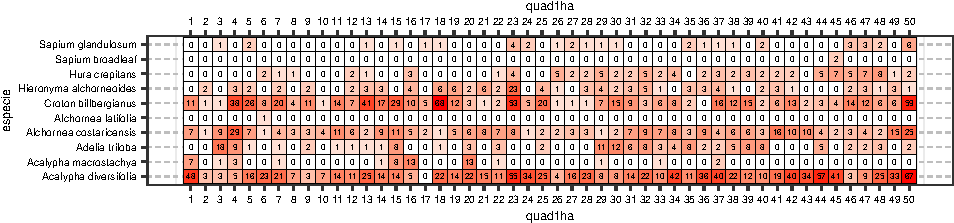
\includegraphics{manuscrito_files/figure-latex/unnamed-chunk-3-1.pdf}
\caption{\label{fig:abun_sp_q}Abundancia por especie por quadrat}
\end{figure}

Desde otra perspectiva, tambien se presentan la riqueza por cuadrículas
en un mapa interactivo pero las especies no estan ordenadas de forma
longitudinal, mas bien de desde el esquema original de trabajo, pero
coincidiendo en parte con la temática anterior donde la intensidad del
color refleja mayor abundancia, y donde cada cuadricula posse el nύmero
de individuos encontrados en esa zona. Antes de pasar el mapa
interactivo aclarar que de forma porvechosa este proyecta el relieve de
la zona donde esta ubicada la parcela de trabajo, lo que abre una puerta
a mas factores determinantes que influyen el la presencia, distribución
y riqueza de las especies, Por qué? pues recordemos que la variación del
relieve influye directamente el clima, humedad, suelo, temperarura y
muchos mas factores que son imprescindibles para la presencia de ciertas
especies, esto a aplica para todo ser vivo, no de forma exlusiva a
Euphorbiaceae.

(ver figura \ref{fig:cuadro_de_riqueza_familia}Riqueza por familia)

\begin{figure}
\centering
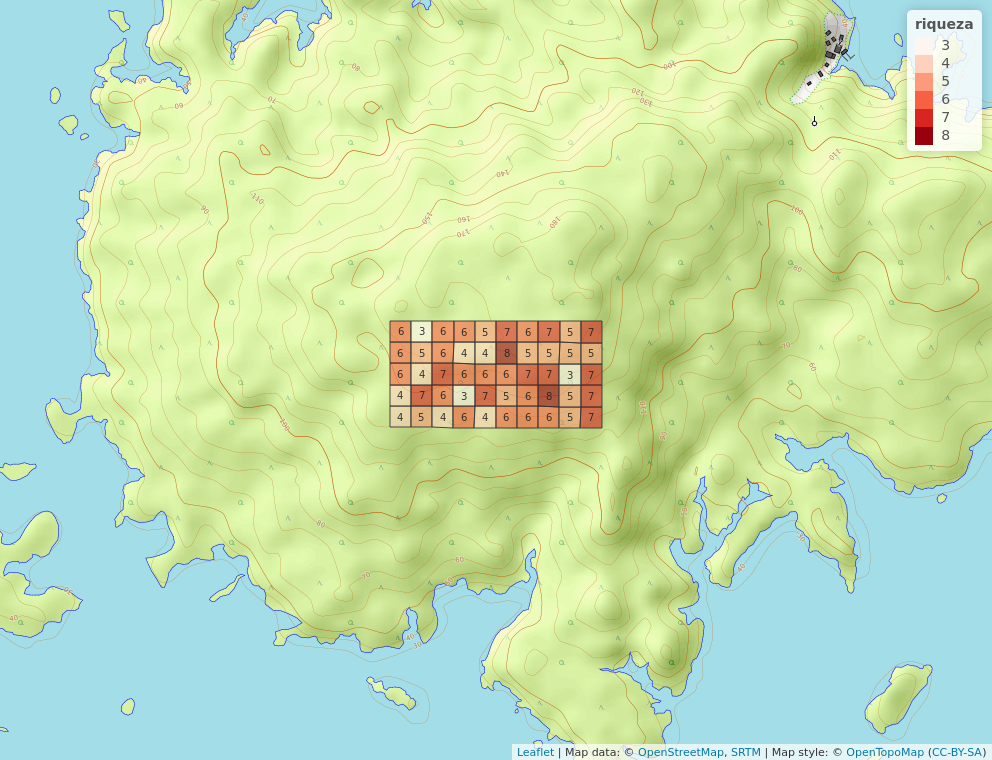
\includegraphics[width=0.50000\textwidth]{mapa_cuadros_riq_mi_familia.png}
\caption{\label{fig:cuadro_de_riqueza_familia}Representacion de la
riqueza de la familia Euphorbiaceae por cuadricula de una hectarea}
\end{figure}

OJO PAMELA!!! ( En resultados recuerda resaltar si la abundancia de
especies de euphorbeacia resulta comun,(``normla'')en panamá a pesar de
ser intertropical, cuando su mayor distribucuin es tropical)

\ldots

\section{Discusión}\label{discusiuxf3n}

\section{Agradecimientos}\label{agradecimientos}

\section{Información de soporte}\label{informaciuxf3n-de-soporte}

\ldots

\section{\texorpdfstring{\emph{Script}
reproducible}{Script reproducible}}\label{script-reproducible}

\ldots

\section*{Referencias}\label{referencias}
\addcontentsline{toc}{section}{Referencias}

\hypertarget{refs}{}
\hypertarget{ref-condit1998tropical}{}
Condit, R. (1998). \emph{Tropical forest census plots: Methods and
results from barro colorado island, panama and a comparison with other
plots}. Springer Science \& Business Media.




\newpage
\singlespacing 
\end{document}
